\documentclass[usenames, dvipsnames, spanish, c]{beamer}

\usepackage[utf8]{inputenc}
% \usepackage[spanish, mexico]{babel}
\usepackage{amsmath}
\usepackage{mathtools}
\usepackage{hyperref}
\usepackage{xcolor}
% \usepackage{color}
\usepackage{ragged2e}
\usepackage{mathrsfs}
% \usepackage{csquotes}
% \usepackage{listings}
\usepackage[scaled]{beramono}
\usepackage[T1]{fontenc}
\usepackage{graphicx}
\usepackage{booktabs}
\usepackage{physics}
\usepackage{minted}
\usepackage{tcolorbox}
\usepackage{tikz}
\usepackage{relsize}
\usepackage{algorithm}
\usepackage{algpseudocode}
\usepackage[shortlabels]{enumitem}
\usepackage{pifont}

\newcommand{\cmark}{\ding{51}}%
\newcommand{\xmark}{\ding{55}}%

\setlist[itemize]{label=\textbullet}  % global enumitem for default itemize

\tcbuselibrary{minted, skins}

\usetikzlibrary{arrows, automata, positioning, fit, shapes.geometric, backgrounds}
  
  \tikzset{
    stylename/.style={
      ->, %arrow type
      >=stealth', %arrow head type (bold)
      shorten >=1pt, 
      auto,
      %semithick,
      initial text=$ $, %no start text
    }
  }

\renewcommand{\indent}{\hspace*{2em}}

\newcommand\CC{C\nolinebreak[4]\hspace{-.05em}\raisebox{.4ex}{\relsize{-3}{\textbf{++}}}~}
\newcommand{\bigO}{\mathcal{O}}

\renewcommand{\Comment}[2][.55\linewidth]{%
  \leavevmode\hfill\makebox[#1][l]{\fontfamily{cmss}\selectfont\color{red}\footnotesize$\longrightarrow$\quad#2}}
% \usepackage{tikz}

% \usetikzlibrary{fit, shapes, arrows}

% \usepackage{courier}
% \usepackage{subfigure}
% \usepackage{enumerate}
% \usepackage{algorithmic}
% \usepackage{algorithm}

% \usepackage{listings}
% \usepackage{lstlinebgrd}

\usetheme{Boadilla}
\usefonttheme[onlymath]{serif}

\newcommand\blfootnote[1]{%
\begingroup
\renewcommand\thefootnote{}\footnote{#1}%
\addtocounter{footnote}{-1}%
\endgroup
}

\algrenewcommand\alglinenumber[1]{\footnotesize #1}

\makeatletter
% start with some helper code
% This is the vertical rule that is inserted
\newcommand*{\algrule}[1][\algorithmicindent]{%
  \makebox[#1][l]{%
    \hspace*{.2em}% <------------- This is where the rule starts from
    \vrule height .75\baselineskip depth .25\baselineskip
  }
}

\newcount\ALG@printindent@tempcnta
\def\ALG@printindent{%
    \ifnum \theALG@nested>0% is there anything to print
    \ifx\ALG@text\ALG@x@notext% is this an end group without any text?
    % do nothing
    \else
    \unskip
    % draw a rule for each indent level
    \ALG@printindent@tempcnta=1
    \loop
    \algrule[\csname ALG@ind@\the\ALG@printindent@tempcnta\endcsname]%
    \advance \ALG@printindent@tempcnta 1
    \ifnum \ALG@printindent@tempcnta<\numexpr\theALG@nested+1\relax
    \repeat
    \fi
    \fi
}
% the following line injects our new indent handling code in place of the default spacing
\patchcmd{\ALG@doentity}{\noindent\hskip\ALG@tlm}{\ALG@printindent}{}{\errmessage{failed to patch}}
\patchcmd{\ALG@doentity}{\item[]\nointerlineskip}{}{}{} % no spurious vertical space
% end vertical rule patch for algorithmicx
\makeatother
%

% Sets the templates
\definecolor{navyblue}{RGB}{0, 0, 128}
\definecolor{crimson}{RGB}{128, 16, 0}

\setbeamertemplate{navigation symbols}{}
\setbeamertemplate{headline}{}
\setbeamertemplate{title page}[default][colsep=-4bp,rounded=true]
\setbeamertemplate{footline}[frame number]
\setbeamertemplate{bibliography item}[text]
\setbeamertemplate{theorems}[numbered]

\setbeamercolor{title}{fg=navyblue, bg=white}
\setbeamercolor{frametitle}{fg=navyblue, bg=white}
\setbeamercolor{structure}{fg=navyblue}
\setbeamercolor{button}{fg=white,bg=navyblue}

\setbeamercovered{transparent}

\tcbset{cppexample/.style={%
    colback=green!5,
    colframe=green!30!black,
    listing only,
    fonttitle=\bfseries,
    listing engine=minted,
    minted language=c++,
    enhanced,
    overlay={\begin{tcbclipinterior}\fill[red!25!green!25!white] (frame.south west)rectangle ([xshift=4mm]frame.north west);\end{tcbclipinterior}}
}}

\tcbset{cppfullexample/.style={%
    % colback=green!5,
    % colframe=green!30!black,
    listing only,
    fonttitle=\bfseries,
    listing engine=minted,
    minted language=c++,
    enhanced,
    overlay={\begin{tcbclipinterior}\fill[black!20!white] (frame.south west)rectangle ([xshift=4mm]frame.north west);\end{tcbclipinterior}}
}}

\tcbset{cppfullborderless/.style={%
    % colback=green!5,
    % colframe=green!30!black,
    listing only,
    listing engine=minted,
    minted language=c++,
    enhanced,
    overlay={\begin{tcbclipinterior}\fill[black!20!white] (frame.south west)rectangle ([xshift=4mm]frame.north west);\end{tcbclipinterior}}
}}

\title{Árboles Binarios de Búsqueda (\textit{Binary Search Trees})}
\subtitle{Programación de Estructuras de Datos y Algoritmos Fundamentales \\ (TC1031)}
\author{
    \texorpdfstring{
        \begin{center}
            M.C. Xavier Sánchez Díaz \\
            \href{mailto:sax@tec.mx}{\texttt{sax@tec.mx}}
        \end{center}
    }
    {M.C. Xavier Sánchez Díaz}
}

\institute[Tecnológico de Monterrey]{
\includegraphics[scale=0.5]{../img/logo}}
\date{}

\begin{document}

\setlength{\rightskip}{0pt}

\begin{frame}[plain]
    \titlepage        
\end{frame}

\begin{frame}{Outline}
    \tableofcontents
\end{frame}

\section{Árboles}

\begin{frame}{¿Qué es un árbol?}{Árboles}
    Un \alert{árbol} es una \textbf{estructura de datos} {\color{Green} jerárquica} y {\color{blue} recursiva}:

    \bigskip

    \begin{itemize}
        \item {\color{Green} Jerárquica} porque tiene \textit{niveles} o \textit{prioridades}
        \item {\color{blue} Recursiva} porque puede describirse recursivamente: \textit{el hijo del hijo del hijo\dots}
    \end{itemize}

    \begin{center}
        
\includegraphics[width=0.3\textwidth]{seventh.jpg}
    \end{center}
\end{frame}

\begin{frame}{Árboles}
    \begin{center}
        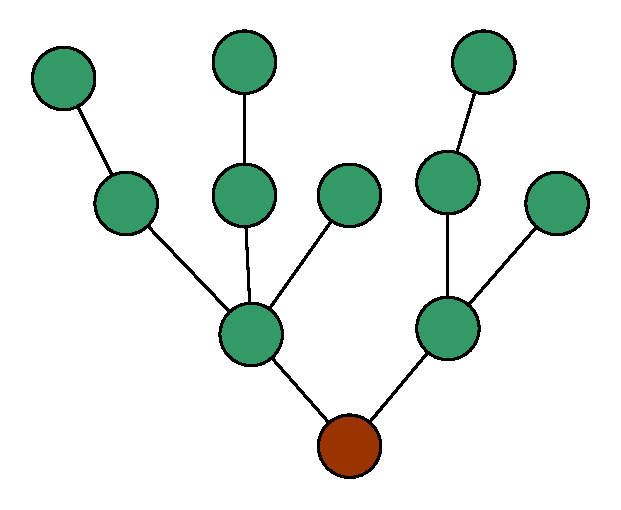
\includegraphics[width=0.75\textwidth]{tree.pdf}
    \end{center}
\end{frame}b

\subsection{Elementos de un árbol}

\begin{frame}{Raíz}{Elementos de un árbol}
    La \alert{raíz} es el \textit{inicio} del árbol; el \textbf{nodo} que es padre de todos.

    \bigskip

    \begin{center}
        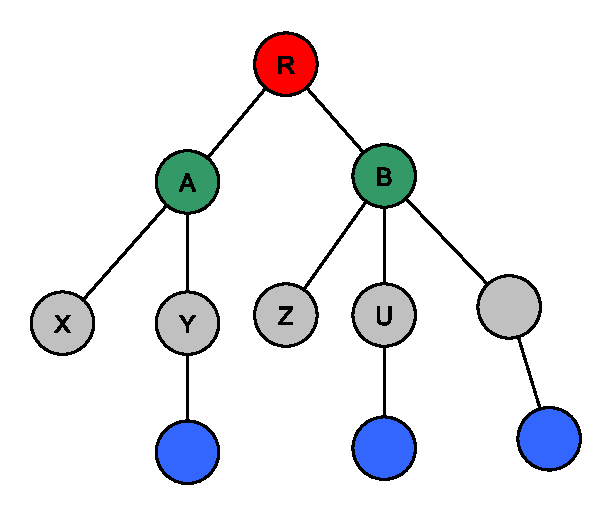
\includegraphics[width=0.6\textwidth]{naming.pdf}
    \end{center}
\end{frame}

\begin{frame}{Nodos y relaciones}{Elementos de un árbol}
    El elemento $R$ es \alert{padre} (\textit{parent}) de los \textbf{nodos} $A$ y $B$. $A$ y $B$ son \alert{hijos} (\textit{children}) de $R$. $A$ y $B$ son hermanos (\textit{siblings}).

    \bigskip

    \begin{center}
        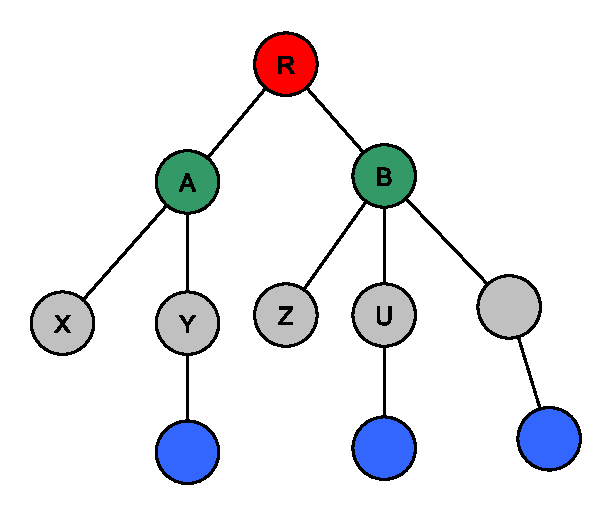
\includegraphics[width=0.6\textwidth]{naming.pdf}
    \end{center}
\end{frame}

\begin{frame}{Niveles}{Elementos de un árbol}
    {\color{Green} $A$} y {\color{Green} $B$} están en el mismo \alert{nivel}. {\color{Gray}$X, Y, Z$} y {\color{Gray}$U$} están en el mismo nivel.

    \bigskip

    \begin{center}
        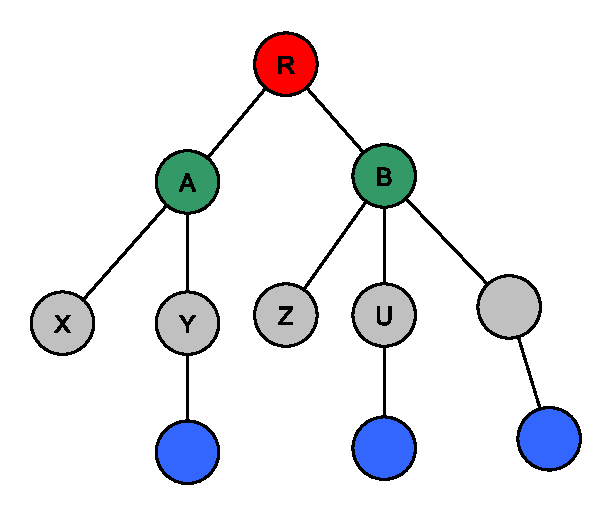
\includegraphics[width=0.6\textwidth]{naming.pdf}
    \end{center}
\end{frame}

\begin{frame}{Jerarquía}{Elementos de un árbol}
    Los {elementos \color{blue} sin descendencia} son los nodos \alert{hoja}.

    \bigskip

    \begin{center}
        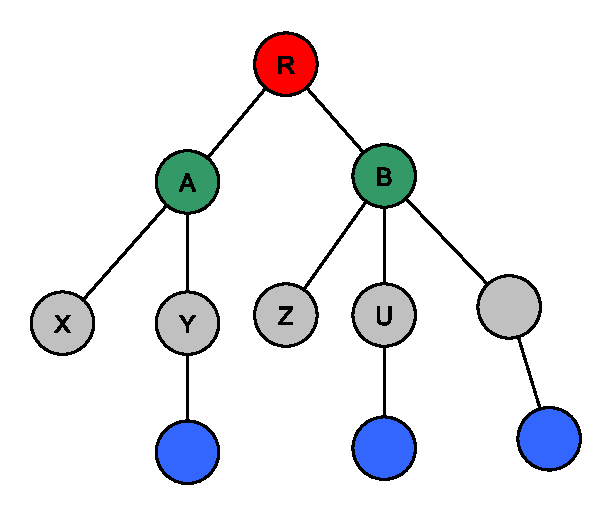
\includegraphics[width=0.6\textwidth]{naming.pdf}
    \end{center}
\end{frame}

\section{Árboles binarios de búsqueda (Binary Search Trees)}

\begin{frame}{Árboles binarios de búsqueda}
Un \alert{árbol binario de búsqueda} (\textit{binary search tree}) es un árbol que es:

\begin{itemize}
    \itemsep3.5ex
    \item \textbf{Binario} porque cada nodo tiene a lo mucho \alert{2} hijos.
    \item \textbf{de Búsqueda} porque como si fuera \textit{binary search}, los descendientes \alert{izquierdos} deben ser \alert{más chicos} que el padre, y los descendientes {\color{blue} derechos} deben ser {\color{blue} más grandes} que el padre.
\end{itemize}

\begin{center}
    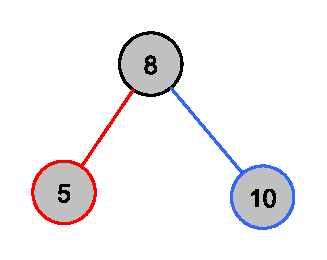
\includegraphics[width=0.3\textwidth]{basecase.pdf}
\end{center}
\end{frame}

\begin{frame}[plain]
    \begin{center}
        \huge
        Teniendo un árbol binario de $n$ nodos donde cada uno (a excepción de las hojas) tuvieran dos hijos cada quién, ¿cuál sería la altura del árbol? es decir, ¿Cuántos niveles tendría?
    \end{center}
\end{frame}

\begin{frame}{Operaciones posibles}{Árboles binarios de búsqueda}
    Las sencillitas:
    \begin{itemize}
        \item Buscar (un valor)
        \item Agregar (un valor)
        \item Borrar (un valor)
    \end{itemize} \pause

    \bigskip

    Las complicadas:
    \begin{itemize}
        \item Obtener la altura (del árbol)
        \item Obtener los ancestros (de un dato)
        \item Obtener el nivel (de un dato)
    \end{itemize} \pause

    \bigskip

    Las \textit{extremadamente} complicadas\footnote{\scriptsize no es cierto}:
    \begin{itemize}
        \item Recorridos (del árbol completo, dado cierto orden)
    \end{itemize}
\end{frame}

\section{Recorridos en árboles (\textit{Walks})}



% \section*{Referencias}

% \begin{frame}[t]{Referencias}
    % \nocite{bibID01}
    % \nocite{bibID02}

    % \bibliographystyle{IEEE}
    % \bibliography{biblio}
% \end{frame}

\end{document}